%!TEX ROOT = ../centralized_vs_distributed.tex

\subsection{\titlecap{stability conditions for discrete-time systems}}\label{app:disc-time-single-int-stability}

\begin{figure}
	\centering
	%!TEX ROOT = ../centralized_vs_distributed.tex

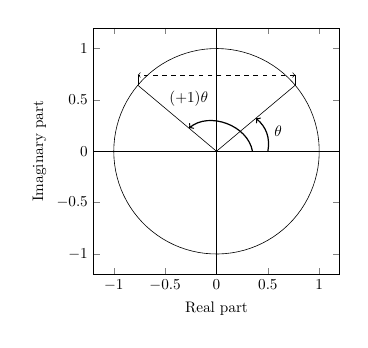
\begin{tikzpicture}[scale=.55]
	\begin{axis}[
		xlabel = Real part,
		ylabel = Imaginary part,
		axis equal image,
		ymin = -1.2,
		ymax = 1.2,
		xmin = -1.2,
		xmax = 1.2]
		\addplot [domain=-180:180, samples=100] ({cos(x)},{sin(x)});
		\draw (-1.2,0) -- (1.2,0);
		\draw (0,-1.2) -- (0,1.2);
		\draw (0,0) -- ({cos(40)},{sin(40)});
		\draw (0,0) -- ({-cos(40)},{sin(40)});
		\path[->,thick] (.5,0) edge[bend right] node [left] {}  ({.5*cos(40)},{.5*sin(40)});
		\path[->,thick] (.35,0) edge[bend right=60] node [left] {}  ({-.35*cos(40)},{.35*sin(40)}) ;
		\node at (.6,.2) {$ \delayn \theta $};
		\node at (-.27,.51) {$ (\delayn+1) \theta $};	
		\draw[<->,dashed] ({cos(40)},{sin(40)+.1}) -- ({-cos(40)},{sin(40)+.1});
		\draw ({cos(40)},{sin(40)+.1}) -- ({cos(40)},{sin(40)});
		\draw (-{cos(40)},{sin(40)+.1}) -- (-{cos(40)},{sin(40)});
		\node at (0.05,{sin(40)+.2}) {$ \gpos $};
	\end{axis}
\end{tikzpicture}
	\caption{A solution of~\eqref{eq:disc-time-single-int-uint-poles-system} in the complex plane.}
	\label{fig:disc-time-single-int-unit-poles}
\end{figure}

\myParagraph{\titlecap{General case}}
In the following, we replace $ \taun $ with $ \delayn $ % drop the subscript from $ \taun $
for the sake of readability.
For the single-integrator case, decoupling the error dynamics yields scalar subsystems of the form
\begin{equation}\label{eq:disc-time-single-int-decoupled}
	\xtilde{}{k+1} = \xtilde{}{k} - \gpos\xtilde{}{k-\tau} + \noisetilde{}{k}.
\end{equation}
The characteristic polynomial $ h(z) $ of~\eqref{eq:disc-time-single-int-decoupled} is obtained by
applying the lag operator $ z $
such that $ \xtilde{}{k}h(z) = \noisetilde{}{k} $,
\begin{equation}\label{eq:disc-time-single-int-characteristic-polinomial}
	h(z) = z - 1 + \gpos z^{-\tau}.
\end{equation}
Similarly, the double-integrator decoupled subsystems are
\begin{equation}\label{eq:disc-time-double-int-decoupled}
%	\xtilde{i}{k+1} = (2-\gvel)\xtilde{i}{k} - (1-\gvel)\xtilde{i}{k-1} - \gvel\gpos\xtilde{i}{k-\taun-1} + \noisetilde{i}{k}
	\begin{aligned}
		\xtilde{}{k+1} &= \xtilde{}{k} + \ztilde{}{k}\\
		\ztilde{}{k+1} &= (1-\gvel)\ztilde{}{k} - \gvel\gpos\xtilde{}{k-\tau} + \noisetilde{}{k},
	\end{aligned}
\end{equation}
with characteristic polynomial
\begin{equation}\label{eq:disc-time-double-int-characteristic-polinomial}
	h(z) = z-2+\gvel+(1-\gvel)z^{-1}+\gvel\gpos z^{-\tau-1}.
\end{equation}
For positive $ \gpos $, stability of~\eqref{eq:disc-time-single-int-decoupled}--\eqref{eq:disc-time-double-int-decoupled}
can be assessed via the Jury stability criterion,
which provides necessary and sufficient conditions for
the roots of~\eqref{eq:disc-time-single-int-characteristic-polinomial} and~\eqref{eq:disc-time-double-int-characteristic-polinomial}
to lie inside the unit circle %in the complex plane
in the form of inequalities involving the coefficients of $ h(z) $.
Being the latter polynomial in $ \gvel $ and $ \gpos $,
the Jury criterion %applied to~\eqref{eq:disc-time-single-int-model}--\eqref{eq:disc-time-double-int-model}
yields $ \Theta(N\tau) $ polynomial inequalities in the feedback gains,
which can be computed through standard software tools.

\myParagraph{Proof of~\cref{prop:disc-time-single-int-stability}}
\cref{eq:disc-time-single-int-characteristic-polinomial} can be studied as a root locus
by varying the gain $ \gpos $.
In particular, $ \gpos = 0 $ yields
a multiple root at $ z_1^* = 0 $ and a simple root at $ z_2^* = 1 $.
Negative values of $ \gpos $ are discarded as they push the latter outside the unit circle.
As $ \gpos $ increases,
the branches leave the unit ball along their asymptotes.
%Notice that, in view of the structure of the root locus,
The admissible values for $ \gpos $ are upper bounded by a threshold gain $ \gpos_{\textit{th}} $
beyond which some roots leave the unit ball.
In particular, we are interested in the minimum gain for which at least one root lies exactly on the unit circle.
Thus, we are looking for roots of~\eqref{eq:disc-time-single-int-characteristic-polinomial}
of the form $ z = \e^{j\theta} $,
\begin{equation}\label{eq:disc-time-single-int-unit-poles-eq}
	\e^{j(\delayn+1)\theta} - \e^{j\delayn\theta} + \gpos = 0.
\end{equation}
\cref{eq:disc-time-single-int-unit-poles-eq} can be equivalently written as the system
\begin{equation}\label{eq:disc-time-single-int-uint-poles-system}
	\begin{cases}
		\cos((\delayn+1)\theta) - \cos(\delayn\theta) + \gpos = 0\\
		\sin((\delayn+1)\theta) = \sin(\delayn\theta).
	\end{cases}
\end{equation}
\autoref{fig:disc-time-single-int-unit-poles} depicts a solution of~\eqref{eq:disc-time-single-int-uint-poles-system} for $ \sin(\delayn\theta) > 0 $.
The case $ \sin(\delayn\theta)<0 $ is analogous
and is omitted.
Further, the solution $ (\delayn+1)\theta = \delayn\theta $
can be discarded because it implies $ \gpos = 0 $ and thus prevents asymptotic stability.
%On the other hand, 
%Therefore, we only focus on the case $ \sin(\delayn\theta)>0 $. % depicted in the left box in~\autoref{fig:disc-time-single-int-unit-poles}.
From basic trigonometric arguments (c.f.~\autoref{fig:disc-time-single-int-unit-poles}),
the second equation in~\eqref{eq:disc-time-single-int-uint-poles-system} implies
\begin{equation}\label{eq:disc-time-single-int-theta}
	\delayn\theta + \dfrac{\theta}{2} = \dfrac{\pi}{2} + 2k\pi \ \longrightarrow \ \theta = \dfrac{\pi+4k\pi}{2\delayn+1}, \quad 
\end{equation}
where we impose $ \theta \in [0,\pi] $
and thus $ k\in\{0,\dots,\floor{\nicefrac{\delayn}{2}}\} $.
This includes all possible cases,
because the roots of~\eqref{eq:disc-time-single-int-characteristic-polinomial} come in complex conjugates pairs.
From~\eqref{eq:disc-time-single-int-theta},
the first equation in~\eqref{eq:disc-time-single-int-uint-poles-system},
and the fact $ \cos((\delayn+1)\theta) = - \cos(\delayn\theta) $,
we retrieve
\begin{equation}\label{eq:disc-time-single-int-unit-roots-gain}
	\gpos = 2\cos\left(\dfrac{\pi\delayn+4k\pi\delayn}{2\delayn+1}\right).
\end{equation}
The right-hand term in~\eqref{eq:disc-time-single-int-unit-roots-gain} is monotone increasing in $ k $.
Indeed, taking the argument of the cosine modulus $ 2\pi $ yields
\begin{equation}\label{eq:disc-time-single-int-angle-modulus}
	\dfrac{\pi\delayn+4k\pi\delayn}{2\delayn+1} \ \mod \ 2\pi = \dfrac{\pi\delayn-2k\pi}{2\delayn+1} \in \left[0,\dfrac{\pi}{2}\right),
\end{equation}
which is nonnegative and monotone decreasing in $ k $ for any $ \tau $.
Finally, the upper bound for the gain $ \gpos $ is given by
\begin{equation}\label{eq:disc-time-single-int-threshold-gain}
	\gpos_{\textit{th}} = \min_k2\cos\left(\dfrac{\pi\delayn+4k\pi\delayn}{2\delayn+1}\right) = 2\cos\left(\dfrac{\pi\delayn}{2\delayn+1}\right).
% 2\sin\left(\dfrac{\pi}{2}\dfrac{1}{2\delayn+1}\right)
\end{equation}


